% First and Second Exams


% Availability

\newcommand{\qAvailabilityOne}{
\begin{ClosedQuestion}
    The stimulus of an availability scenario is
        
    \optionA{A failure.}
    \optionB{An error.}
    \optionC{A fault.}
    \optionD{An input.}
 \putOptions 
\end{ClosedQuestion}
}

\newcommand{\qAvailabilityTwo}{
\begin{ClosedQuestion}
    An availability tactic to prevent faults is 
        
    \optionA{Increase competence set.}
    \optionB{Shadow.}
    \optionC{Voting.}
    \optionD{Ignore faulty behavior.}
 \putOptions 
\end{ClosedQuestion}
}


% Performance

\newcommand{\qPerformanceOne}{
\begin{ClosedQuestion}
    A response measure of a performance scenario is 
        
    \optionA{Stochastic event.}
    \optionB{Overload.}
    \optionC{Change level of service.}
    \optionD{Throughput.}
 \putOptions 
\end{ClosedQuestion}
}

\newcommand{\qPerformanceTwo}{
\begin{ClosedQuestion}
    A performance tactic to control resource demand is 
        
    \optionA{Increase resources.}
    \optionB{Reduce overhead.}
    \optionC{Bound queue sizes.}
    \optionD{Introduce concurrency.}
 \putOptions 
\end{ClosedQuestion}
}

% Modifiability

\newcommand{\qModifiabilityExamOne}{
\begin{ClosedQuestion}
    The layered architectural style applies the modifiability architectural tactic of
        
    \optionA{Split module.}
    \optionB{Use an intermediary.}
    \optionC{Restrict dependencies.}
    \optionD{Refactor.}
 \putOptions 
\end{ClosedQuestion}
}

\newcommand{\qModifiabilityExamTwo}{
\begin{ClosedQuestion}
    A response measure of a modifiability scenario is
        
    \optionA{When the modification should occur.}
    \optionB{The features that will be implemented.}
    \optionC{The new defects introduced.}
    \optionD{Defer binding.}
 \putOptions 
\end{ClosedQuestion}
}


% Module viewtype

\newcommand{\qModuleViewtypeExamOne}{
\begin{ClosedQuestion}
    One of the advantages of having views of the module viewtype is that they allow to do an impact analysis to predict the effect of modifying the system. The architectural style of the module viewtype which provides richer information for this impact analysis is
        
    \optionA{Decomposition style.}
    \optionB{Uses style.}
    \optionC{Generalization style.}
    \optionD{Layered style.}
 \putOptions 
\end{ClosedQuestion}
}

\newcommand{\qModuleViewtypeExamTwo}{
\begin{ClosedQuestion}
    One of the advantages of having views of the module viewtype is that they allow to do a traceability analysis of requirements, how the functional requirements of the system are supported by module responsibilities. The modifiability tactic that is involved in this mapping is
        
    \optionA{Split module.}
    \optionB{Abstract common services.}
    \optionC{Restrict dependencies.}
    \optionD{Encapsulation.}
 \putOptions 
\end{ClosedQuestion}
}


% Module styles

\newcommand{\qDecompositionGeneralization}{
\begin{ClosedQuestion}
  Consider that a chess game should
  provide an automatic and intelligent chess player, and that to
  implement that player we will use some of the many chess engines
  already available in the market.  Moreover, the system should allow
  the user to choose which engine to use for each new game.  Given
  these requirements, which of the architectural styles from the
  module viewtype are best suited to satisfy them?
 
  \optionA{The Decomposition style.}
  \optionB{The Decomposition and Uses styles.}
  \optionC{The Layered style.}
  \optionD{The Generalization and Decomposition styles.}
 \putOptions 
\end{ClosedQuestion}
}

\newcommand{\qDVDCatalogMobile}{
\begin{ClosedQuestion}
    Consider the module viewtype views of the Catalog of DVD application. The architect knows about a new requirement 
    
    \begin{quote}
        To support iPhone/iPad/Android version with sync, which allows offline use of the application in the mobile device and data synchronization to occur when a connection is available
    \end{quote}
    
    This requirement requires a change of
    
    \optionA{The decomposition view to include a module for the synchronization responsibilities}
    \optionB{The uses view to represent how the mobile device uses the Catalog application}
    \optionC{The layered view to include a layer for each type of device}
    \optionD{The domain layer of the layered style to represent the types of devices}
 \putOptions
\end{ClosedQuestion}
}


% Component-and-Connector viewtype

\newcommand{\qComponentAndConnectorViewtypeOne}{
\begin{ClosedQuestion}
    In the component-and-connector viewtype connectors can be complex, which means that they provide a rich set of qualities to the interaction between the components that they connect. These complex connectors can be documented in another view using a set of components interacting through simpler connectors.
        
    \optionA{Whenever complex connectors are used in architectural views it is necessary to also document their decomposition.}
    \optionB{It is preferable to only design views that do not use complex connectors to increase understandability.}
    \optionC{If there is some technology available that implements the complex connectors it is not necessary to document their decomposition.}
    \optionD{Whenever possible it should be avoided to use complex connectors because developers have difficult to know how to implement them.}
 \putOptions 
\end{ClosedQuestion}
}

\newcommand{\qComponentAndConnectorViewtypeTwo}{
\begin{ClosedQuestion}
    Considered the following two views of a system that receive a stream of character and produce the same stream where the characters are alternately uppercase and lowercase.
    
    \begin{center}
       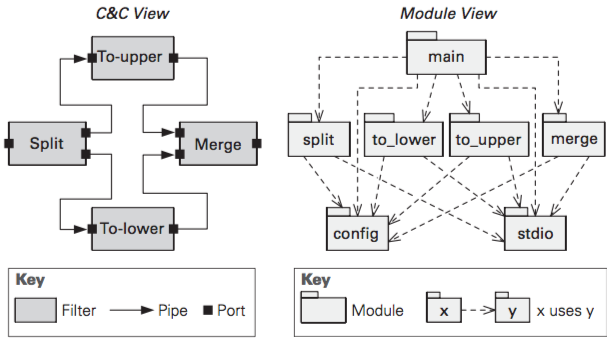
\includegraphics[width=120mm]{1-module-and-cc}
    \end{center}
        
    \optionA{The \emph{config} module is not used in the implementation of any component.}
    \optionB{The \emph{main} module is used in the implementation of all components.}
    \optionC{The connectors only use the \emph{stdio} module for their implementation.}
    \optionD{The \emph{Split} component uses the \emph{to\_lower} module for its implementation}
 \putOptions 
\end{ClosedQuestion}
}


% Component-and-Connector style

\newcommand{\qPublishsubscribeOne}{
  \begin{ClosedQuestion}
      Typically, Instant Messaging clients have a window to list the contacts of the user, and
      show in that window the status of each contact (whether it is available, unavailable, busy,
      etc). Given that the status of a contact may be changed at any time, and that the contact's
      status is given by the Instant Messaging application of that contact, which architectural
      style represents best the interaction pattern between these components?

       \optionA{The Shared Data style.}
       \optionB{The Pipes-and-filters style.}
       \optionC{The Publish-subscribe style.}
      \optionD{The Client-Server style.}
   \putOptions

  \end{ClosedQuestion}
}

\newcommand{\qPipesFilters}{
\begin{ClosedQuestion}
    Consider that you intend to develop a system where it is necessary to change the emails received by the server (for instance, to remove potential virus or URLs for phishing sites). The goal is that each email is processed by this system before it is sent to other servers or it is stored locally. Additionally, the system should be easily modified to support new kinds of transformations. Which style is more suitable to satisfy these requirements? 

    \optionA{Peer-to-Peer.}
    \optionB{Pipe-and-Filter.}
    \optionC{Client-Server.}
    \optionD{Publish-Subscribe.}
 \putOptions
\end{ClosedQuestion}
}

% Architectures for scalable web applications

\newcommand{\qProxyServer}{
\begin{ClosedQuestion}
    Consider the following figure that presents a Proxy Server that collapses requests from different users.
    
    \begin{center}
        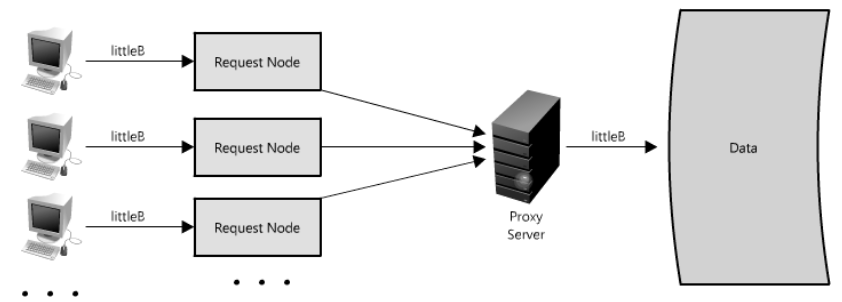
\includegraphics[width=120mm]{1-proxy-server}
    \end{center}
    
    
    \optionA{This solution optimizes the performance in terms of the latency of each request.}
    \optionB{This solution allows an "infinite"\ increase of the number clients by allowing the inclusion of more Request Nodes.}
    \optionC{This solution continues to provide service even if a crash occurs in the Data server.}
    \optionD{This solution optimizes the performance in terms of the throughput of processed requests.}
 \putOptions 
\end{ClosedQuestion}
}

\newcommand{\qScalableArchitectureOne}{
  \begin{ClosedQuestion}
    Consider the following figure that presents a Image Hosting System.
    
    \begin{center}
        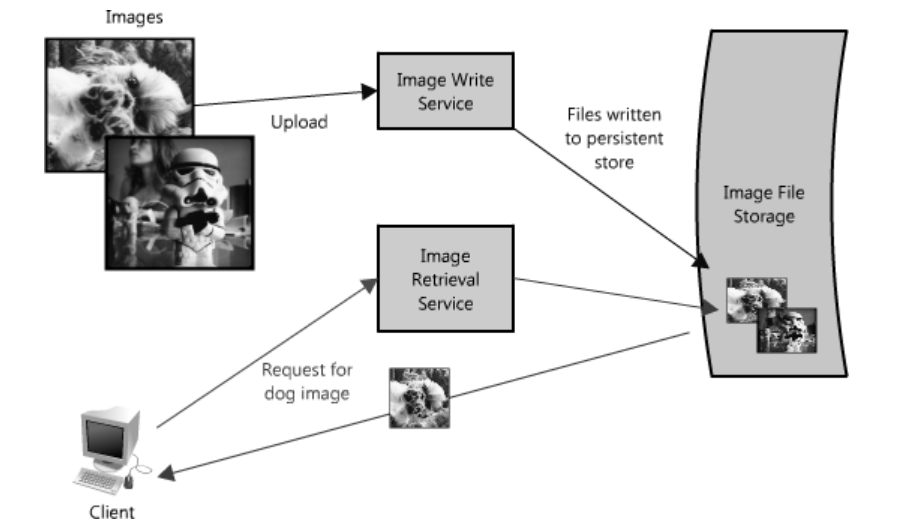
\includegraphics[width=120mm]{1-image-hosting}
    \end{center}
    
    By adding another Image File Storage component, which contains a redundant copy of the data and provides read access to the clients, but without guaranteeing a ACID transactional behavior between reads and writes, it improves the quality(ies) of
    
    \optionA{Performance.}
    \optionB{Availability for incorrect responses from the Image File Storage component.}
    \optionC{Performance and Availability for crashes of the Image File Storage component.}
    \optionD{Performance and Availability for incorrect responses from the Image File Storage component.}
    \putOptions

 \end{ClosedQuestion}
}


% The Architecture of Graphite

\newcommand{\qGraphiteOne}{
\begin{ClosedQuestion}
    Consider the following fragment in the description of the Graphite system.
    
    \begin{quote}
        The Graphite webapp allows users to request custom graphs with a simple URL-based API. Graphing parameters are specified in the query-string of an HTTP GET request, and a PNG image is returned in response. 
    \end{quote}
    
    To describe this scenario it should be designed a view that applies the following architectural style
        
    \optionA{Decomposition.}
    \optionB{Aspects.}
    \optionC{Layered.}
    \optionD{Data model.}
 \putOptions 
\end{ClosedQuestion}
}

\newcommand{\qGraphiteTwo}{
\begin{ClosedQuestion}
      Which quality, or qualities, of the Graphite system are described by the sentence: \emph{Graphite's Composer UI provides a point-and-click method to create a graph from which you can simply copy and paste the URL.}

    \optionA{Usability and Performance.}
    \optionB{Usability.}
    \optionC{Performance.}
    \optionD{Modifiability.}
 \putOptions 
\end{ClosedQuestion}
}


% The Architecture of Catalog of DVDs

\newcommand{\qDVDOne}{
\begin{ClosedQuestion}
    Consider the following usability scenario of the Catalog of DVDs case study
    
    \begin{quote}
        The user intends to have up-to-date info about the movies and the system informs the user that the existing sources have new information about one of his DVDs, which helps to maintain an up-to-date catalog. 
    \end{quote}
    
    The tactic used to fulfill this scenario is
        
    \optionA{Aggregate.}
    \optionB{Maintain user model.}
    \optionC{Maintain task model.}
    \optionD{Maintain system model.}
 \putOptions 
\end{ClosedQuestion}
}

\newcommand{\qDVDTwo}{
\begin{ClosedQuestion}
    Consider the following generalization view of the Catalog of DVD case study to fulfill a modifiability scenario
    
    \begin{center}
        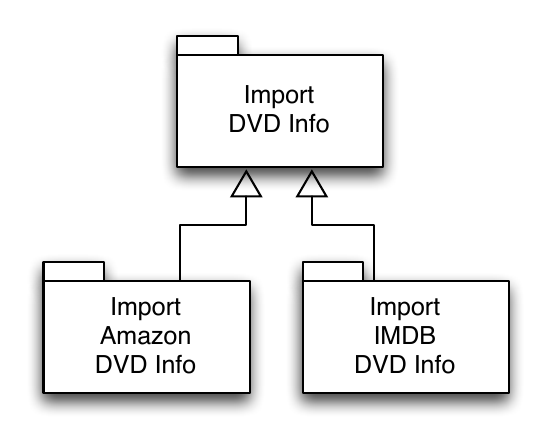
\includegraphics[width=60mm]{1-dvd-generalization}
    \end{center}
    
    From this view the stakeholders can infer
            
    \optionA{The cost of the modification.}
    \optionB{That the integration of a new source will not have any impact on the other modules of the Catalog of DVDs.}
    \optionC{That the impact of integrating a new source is controlled by the interface of \emph{Import DVD Info} Module.}
    \optionD{That the modification can occur at runtime.}
 \putOptions 
\end{ClosedQuestion}
}

% The Architecture of Adventure Builder

\newcommand{\qAdventureBuilderOne}{
\begin{ClosedQuestion}
    Consider the following view of the Adventure Builder case study that applies the tiers architectural style 
    
    \begin{center}
       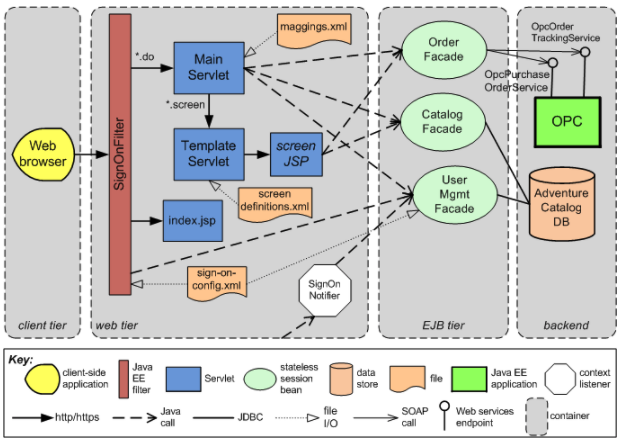
\includegraphics[width=100mm]{1-adventure-tiers}
    \end{center}
        
    \optionA{This view shows that if is possible to scale differently the \texttt{web tier} from the \texttt{EJB tier}.}
    \optionB{This view shows that the \texttt{Adventure Builder Catalog DB} and the \texttt{OPC} components should be deployed in the same hardware.}
    \optionC{This view \textbf{does not} show that the \texttt{Adventure Builder Catalog DB} and the \texttt{OPC} components can execute behind a firewall.}
    \optionD{This view \textbf{does not} show that the access to the \texttt{web tier} has some security qualities.}
 \putOptions
\end{ClosedQuestion}
}

\newcommand{\qAdventureBuilderTwo}{
\begin{ClosedQuestion}
    Consider the following view of the Adventure Builder case study 
    
    \begin{center}
       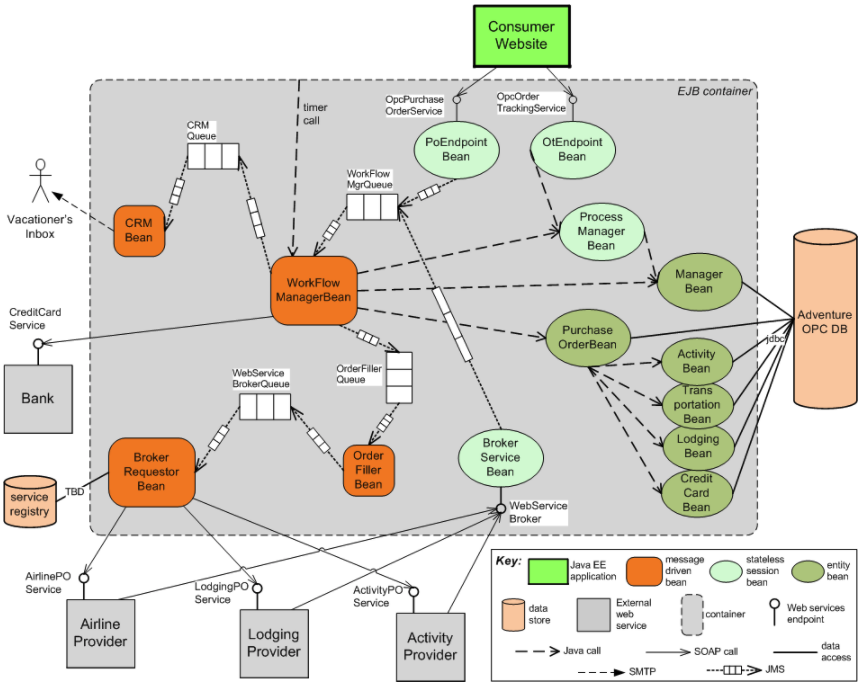
\includegraphics[width=120mm]{1-adventure-com-proc}
    \end{center}
        
    \optionA{This view shows that the processing of orders is done synchronously.}
    \optionB{This view shows that the processing of tracking requests is done synchronously.}
    \optionC{This view shows that bank debits are done asynchronously.}
    \optionD{This view shows that the responses from the providers are processed synchronously.}
 \putOptions
\end{ClosedQuestion}
}

% The Architecture of Pulse

\newcommand{\qPulseOne}{
\begin{ClosedQuestion}
    Consider the following view of the Pulse case study 
    
    \begin{center}
        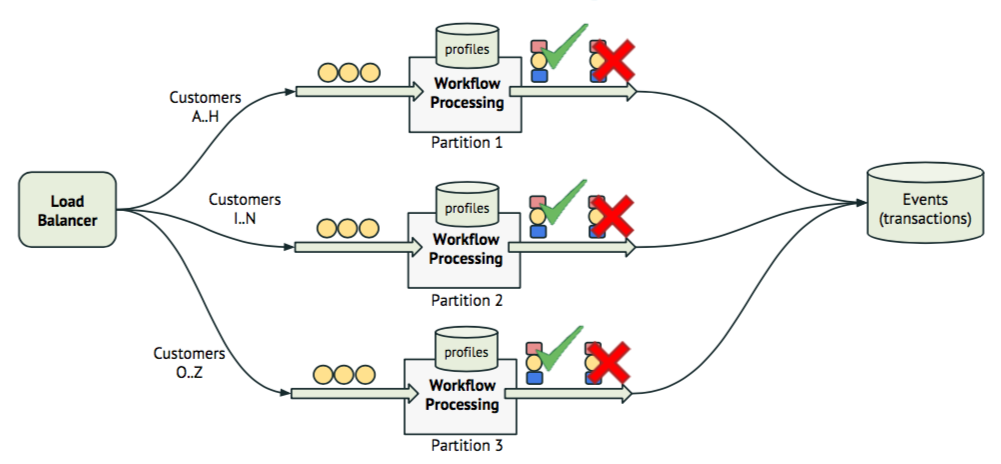
\includegraphics[width=120mm]{1-pulse-multiple-copies-computation}
    \end{center}
    
    This view provides a solution that uses the following tactic
            
    \optionA{Pipe-and-filter.}
    \optionB{Maintain multiple copies of data.}
    \optionC{Maintain multiple copies of computation.}
    \optionD{Introduce concurrency.}
 \putOptions
\end{ClosedQuestion}
}

\newcommand{\qPulseTwo}{
\begin{ClosedQuestion}
    Consider the following view of the Pulse case study 
    
    \begin{center}
        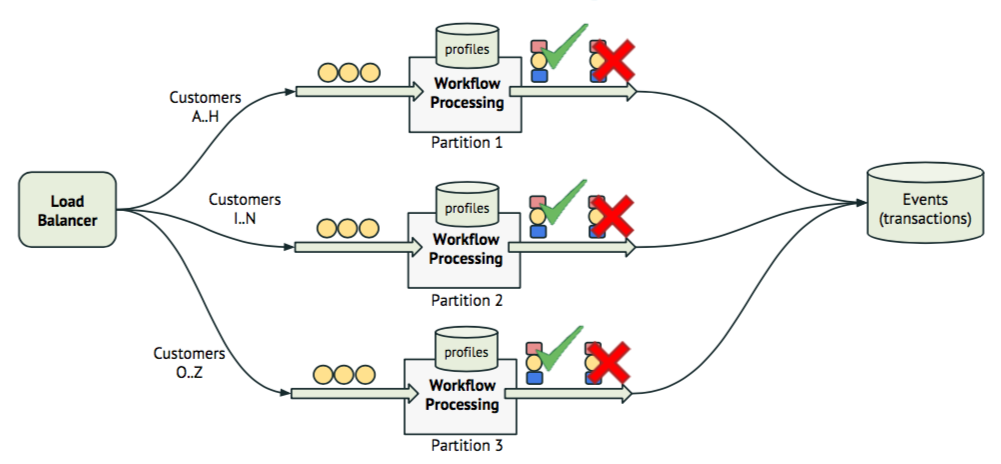
\includegraphics[width=120mm]{1-pulse-multiple-copies-computation}
    \end{center}
    
    This view applies the following architectural styles
            
    \optionA{Pipe-and-filter and tiers.}
    \optionB{Shared-data and publish-subscribe.}
    \optionC{Pipe-and-filter and publish-subscribe.}
    \optionD{Pipe-and-filter and shared-data.}
 \putOptions
\end{ClosedQuestion}
}

% The Architecture of the Morrison's OrderPad

\newcommand{\qOrderPadOne}{
\begin{ClosedQuestion}
    In the description of architecture of the OrderPad case study it can be read that the updates the user does on the OrderPad when it is offline are not lost. This availability quality is achieved through a    

  \optionA{Ignore faulty behaviour tactic}
  \optionB{Ping-and-echo tactic}
  \optionC{Active redundancy tactic}
  \optionD{Retry tactic}
 \putOptions
\end{ClosedQuestion}
}

\newcommand{\qOrderPadTwo}{
\begin{ClosedQuestion}
    Consider the architecture of the Morrison's OrderPad. The connector between the client component, executing in the Pad, and the server component, executing in the OrderPadDatabase
    
    \optionA{Guarantees that the redundant data in the client and the server is always synchronized.}
    \optionB{Implements an event bus that allows the server to inform the client about new order recommendations.}
    \optionC{Do not loose the changes done on the client component if the server is not available.}
    \optionD{It completely hides the server faults from the Pad user.}
 \putOptions
\end{ClosedQuestion}
}

% Architectural Viewtypes and Styles

\newcommand{\qLayered}{
\begin{ClosedQuestion}
    Consider the Uses architectural style of the Module viewtype
        
    \optionA{Cycles in the uses relation between modules are a good sign, because it indicates that several modules should be tested together.}
    \optionB{The project manager uses this view to get advice on the incremental development of the system.}
    \optionC{The uses relation should be applied to the coarse-grained modules, because it allows to identify circular dependences.}
    \optionD{There isn't any relation with the layered architectural style because the allowed-to-use relation is more generic.}
 \putOptions 
\end{ClosedQuestion}
}

\newcommand{\qDataModel}{
\begin{ClosedQuestion}
    In Facebook it is not possible to have the information about more that one bilion users in a single disk. Therefore, a sharding technique is applied, where the persistent information is split between several database servers, and requests are routed to the right servers for queries and updates. Additionally, due to performance requirements, the information needs to be replicated in several servers. To describe this architecture
    
    \optionA{It is not necessary to have any view of the Data Model architectural style because Facebook information has a very simple structure.}
    \optionB{It is enough to design a view of the Data Model architectural style at the conceptual level because Facebook information has a very simple structure.}
    \optionC{It is enough to design a view of the Data Model architectural style at the logical level because the information will be stored in a relational database.}
    \optionD{It is necessary to design a view of the Data Model architectural style at the physical level to deal with performance and consistency issues of the access to data.}
 \putOptions
\end{ClosedQuestion}
}

% Component-and-connector

\newcommand{\qDynamicReconfiguration}{
\begin{ClosedQuestion}
    In the description of the Gnutella system can be read:
    
    \begin{quote}
        The topology of the system changes at runtime as peer components connect and disconnect to the network.
    \end{quote}
    
    \optionA{When a peer connects to the network it establishes connections with all other peers in the network.}
    \optionB{The behavior described in the sentence can be represented in a view where the dynamic reconfiguration architectural style is used.}
    \optionC{When a peer receives a connection it sends all its files to the peer connecting it.}
    \optionD{The behavior described in the sentence can be represented in a view where the tier architectural style is used.}
 \putOptions
\end{ClosedQuestion}
}

\newcommand{\qSOA}{
  \begin{ClosedQuestion}
    Suppose that you are developing the software architecture of a new
    system for an organization composed of several organizational
    units, each one with its own information systems, which have been
    developed independently of each other over the course of several
    years and depending on the particular needs of each unit.  Your
    system has the goal of integrating the various existing systems,
    providing in this way not only a unified view of how the
    organization works, but also allowing the creation of new
    processes within the organization that involve more than one unit.
    Which architectural style is better suited to design such a
    system?

    \optionA{The Decomposition style.}
    \optionB{The Client-Server style.}
    \optionC{The Service Oriented Architecture style.}
    \optionD{The Communicating Processes style.}

    \putOptions

% Resposta: C
 \end{ClosedQuestion}
}

% Allocation

\newcommand{\qDeployment}{
\begin{ClosedQuestion}
  In the software architecture of a system, the Deployment architectural style of the allocation viewtype is
  best suited for

    \optionA{Analysing the performance of the system.}
    \optionB{Planning incremental releases of the system.}
    \optionC{Estimating the effort needed to implement the system.}
    \optionD{Analysing the system's portability and reusability.}
    \putOptions

% Resposta: A
 \end{ClosedQuestion}
}

\newcommand{\qWorkAssigment}{
\begin{ClosedQuestion}
    Consider the Work Assignment architectural style of the allocation viewtype.
            
    \optionA{It assigns components and connectors to people and teams.}
    \optionB{It is useful for the project managers.}
    \optionC{It does not consider the software that is outsourced.}
    \optionD{It allows to estimate the cost of hardware.}
 \putOptions 
\end{ClosedQuestion}
}

% Archictectural variations of web applications 

\newcommand{\qWebAppsOne}{
\begin{ClosedQuestion}
    Consider a web application that was implemented using three layers: presentation, domain logic, and data access. How are these layers mapped into the components if it is a rich interface application.
            
    \optionA{All layers are mapped to the application server component.}
    \optionB{The presentation and domain logic layers are mapped to the application server component and the data access layer to the repository component.}
    \optionC{The presentation layer is mapped to the browser component and the other two layers are mapped to the application server component.}
    \optionD{All layers are mapped to the browser component where the data access layer will contains, besides a module to access a local repository, modules to access external services.}
 \putOptions 
\end{ClosedQuestion}
}

\newcommand{\qWebAppsTwo}{
\begin{ClosedQuestion}
    Consider a web application that supports several types of user interface, e.g., web, mobile, etc. If it has to process a high volume of requests, which depend on the type of user interface, and a multi-tier architecture is followed. How many tiers should be used?
            
    \optionA{One.}
    \optionB{Two.}
    \optionC{Three.}
    \optionD{Four.}
 \putOptions 
\end{ClosedQuestion}
}

% The Architecture of Fénix

\newcommand{\qFenixOne}{
\begin{ClosedQuestion}
    In the context of the FenixEdu case study, the business case was to

    \optionA{Incorporate in the organization's core business the goals of a software house.}
    \optionB{Do in-house development.}
    \optionC{Integrate the development of the software system with the organization's business goals.}
    \optionD{Reimplement all the information systems of the organization}
 \putOptions
\end{ClosedQuestion}
}

\newcommand{\qFenixTwo}{
\begin{ClosedQuestion}
    When applying Attribute-Driven Design (ADD) to the FenixEdu system the creation of a view where there are redundant web servers, load balancers and database servers 

    \optionA{Results from a utility tree for performance.}
    \optionB{Results from a single availability scenario.}
    \optionC{Results from the application of a single ADD iteration.}
    \optionD{Results from the application of several ADD iterations.}
 \putOptions
\end{ClosedQuestion}
}

% Microservices and Aggregates

\newcommand{\qAggregateOne}{
\begin{ClosedQuestion}
    In a microservices architecture, aggregates are used as a unit of processing

    \optionA{An aggregate can contain a large number of instances.}
    \optionB{An aggregate is usually loaded in its entirety from the database.}
    \optionC{An aggregate has runtime references to other aggregates.}
    \optionD{An aggregate is cluster of domain classes.}
 \putOptions
\end{ClosedQuestion}
}

\newcommand{\qAggregateTwo}{
\begin{ClosedQuestion}
    Consider the following decomposition of a domain model into 3 aggregates. If, instead of this decomposition, \texttt{Customer} and \texttt{Order} were in the same aggregate  
    
    \begin{center}
       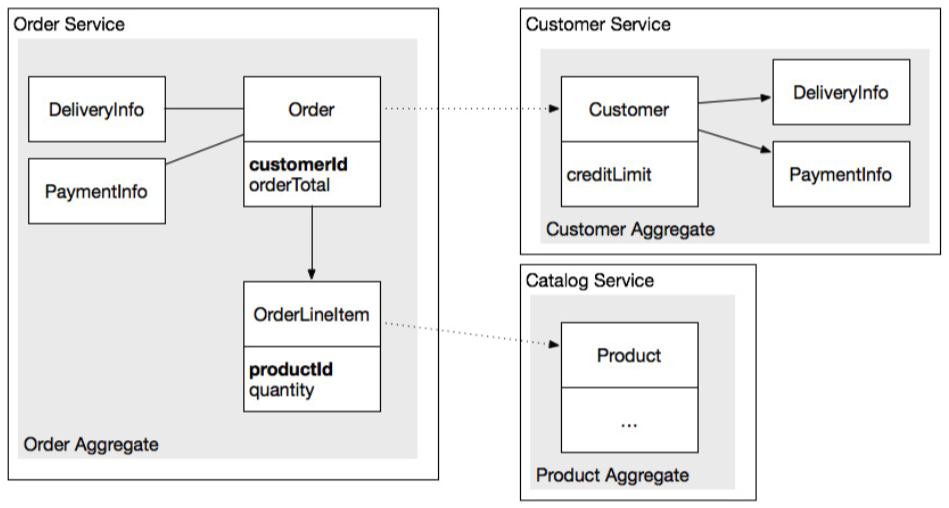
\includegraphics[width=120mm]{1-aggregate}
    \end{center}

    \optionA{It would reduce the scalability for updates of different orders for the same customer.}
    \optionB{Two users would conflict if they attempt to edit different orders for the same customer.}
    \optionC{As the number of orders grows it will be increasingly expensive to load the aggregate.}
    \optionD{All the above.}
 \putOptions
\end{ClosedQuestion}
}

% Microservices and Event Sourcing

\newcommand{\qMicroservicesExamOne}{
\begin{ClosedQuestion}
    Consider the Microservice architectural style. Which of the following sentences \textbf{does not} describe an advantage of microservices?
            
    \optionA{Each service can be developed and deployed independently}
    \optionB{Easier to scale development}
    \optionC{Eliminates any long-term commitment to a technology stack}
    \optionD{Testing is easier}
 \putOptions 
\end{ClosedQuestion}
}

\newcommand{\qMicroservicesExamTwo}{
\begin{ClosedQuestion}
    Consider the following definition of Microservice architectural style by Martin Fowler
    
    \begin{quote}
        The microservice architectural style is an approach to developing a single application as a suite of small services, each running in its own process and communicating with lightweight mechanisms, often an HTTP resource API. These services are built around business capabilities and independently deployable by fully automated deployment machinery. There is a bare minimum of centralized management of these services, which may be written in different programming languages and use different data storage technologies.
    \end{quote}
    
    To represent an architecture based on Microservices 
            
    \optionA{We do not need a view of the module viewtype because it is about the runtime properties of the system.}
    \optionB{We do not need a view of the allocation viewtype because deployment is automated.}
    \optionC{The component-and-connector view should emphasize the performance qualities of systems following the microservices architecture.}
    \optionD{It is necessary to use views of the three viewtypes.}
 \putOptions 
\end{ClosedQuestion}
}


% Fourth Mini-test


% Component-and-connector crosscutting concerns and allocation styles

\newcommand{\qCommunicatingProcesses}{
\begin{ClosedQuestion}
    In the web page of the NGINX HTTP server can be read
    
    \begin{quote}
        NGINX is a free, open-source, high-performance HTTP server and reverse proxy, as well as an IMAP/POP3 proxy server. (...)
        Unlike traditional servers, NGINX doesn't rely on threads to handle requests. Instead it uses a much more scalable event-driven (asynchronous) architecture. This architecture uses small, but more importantly, predictable amounts of memory under load.
    \end{quote}
    
    According to the above description the most adequate architectural style to represent the performance qualities of NGINX is
    
    \optionA{Dynamic Reconfiguration.}
    \optionB{Tiers.}
    \optionC{Communicating Processes.}
    \optionD{Install.}
 \putOptions
\end{ClosedQuestion}
}

\newcommand{\qTiers}{
\begin{ClosedQuestion}
    The Tiers architectural style
    
    \optionA{Applies layers to tiers.}
    \optionB{Restricts the communication between components because, for instance, a group of components should be located in the same hardware.}
    \optionC{Is an extension of the Client-Server architectural style.}
    \optionD{Defines tiers as components.}
 \putOptions
\end{ClosedQuestion}
}

\newcommand{\qAllocationStylesCost}{
\begin{ClosedQuestion}
    Consider a stakeholder that is particularly concerned about the total cost of the project. When it comes to describing the system using allocation viewtypes is interested in

    \optionA{A deployment view.}
    \optionB{A work assignment view.}
    \optionC{A deployment and a work assignment view.}
    \optionD{A install view.}
 \putOptions
\end{ClosedQuestion}
}


% Catalog of DVD

\newcommand{\qDVDTopDecomposition}{
\begin{ClosedQuestion}
    Consider the following decomposition view of the Catalog of DVD case study.
    
    \begin{center}
       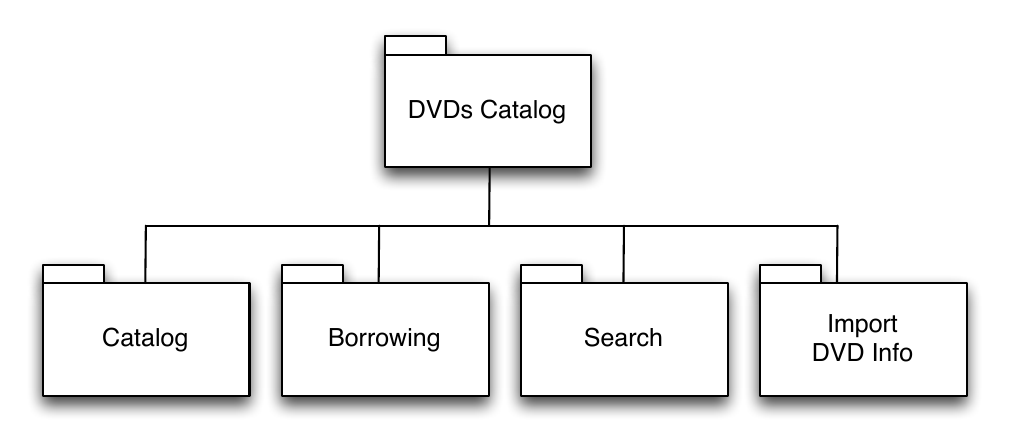
\includegraphics[width=100mm]{dvd-top-decomposition}
    \end{center}

    \optionA{The decomposition was driven by a defer binding tactic.}
    \optionB{The decomposition was driven by a quality that is supported by a restrict dependencies tactic.}
    \optionC{The decomposition was driven by a split module tactic.}
    \optionD{The decomposition was driven by a quality that is supported by an encapsulate tactic.}
 \putOptions
\end{ClosedQuestion}
}

\newcommand{\qDVDAutocomplete}{
\begin{ClosedQuestion}
    Consider the following decomposition views of the Catalog of DVD case study were the \emph{Autocomplete} module is implemented in javascript and executes in a browser.
    
    \begin{center}
    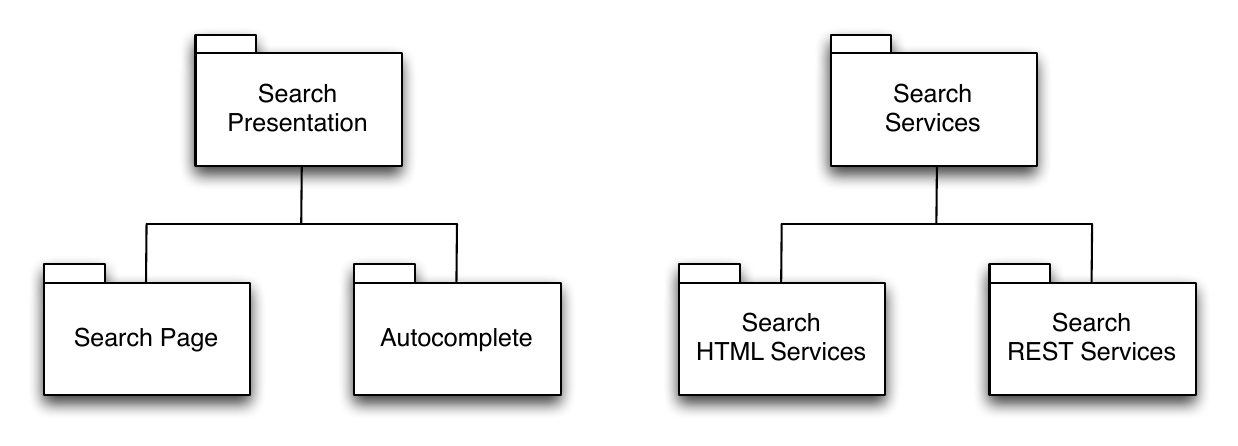
\includegraphics[width=120mm]{dvd-autocomplete}
    \end{center}

    \optionA{The view illustrates the achievement of a security scenario.}
    \optionB{The view illustrates the achievement of a performance scenario.}
    \optionC{The view results from the implementation of a support user initiative tactic.}
    \optionD{The view results from the implementation of a support system initiative tactic.}
 \putOptions
\end{ClosedQuestion}
}

\newcommand{\qDVDGeneralization}{
\begin{ClosedQuestion}
    Consider the following generalization view of the Catalog of DVD case study.
    
    \begin{center}
       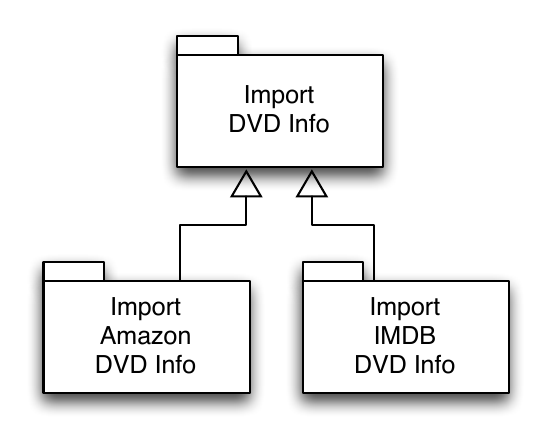
\includegraphics[width=60mm]{dvd-generalization}
    \end{center}

    \optionA{This generalization was driven by a split module tactic.}
    \optionB{This view fulfills an availability scenario, which defines the expected behavior whenever an external source is not available.}
    \optionC{This view fulfills a modifiability scenario, which states about the cost of adding a new source of information to the system.}
    \optionD{This view fulfills a modifiability scenario, which states that it should be easy to support the system in new software platforms, e.g. \emph{Windows} or \emph{OS X} .}
 \putOptions
\end{ClosedQuestion}
}


% Graphite

\newcommand{\qGraphitePerformanceScenario}{
\begin{ClosedQuestion}
    In the context of the \emph{Graphite} case study, consider the following view that represents the internal behavior of the \emph{Carbon} component, where the components \texttt{r1,... , rn, w} are threads and \texttt{q1, ..., qn} are buffers. This view shows the Graphite's architecture support of
    
    \begin{center}
       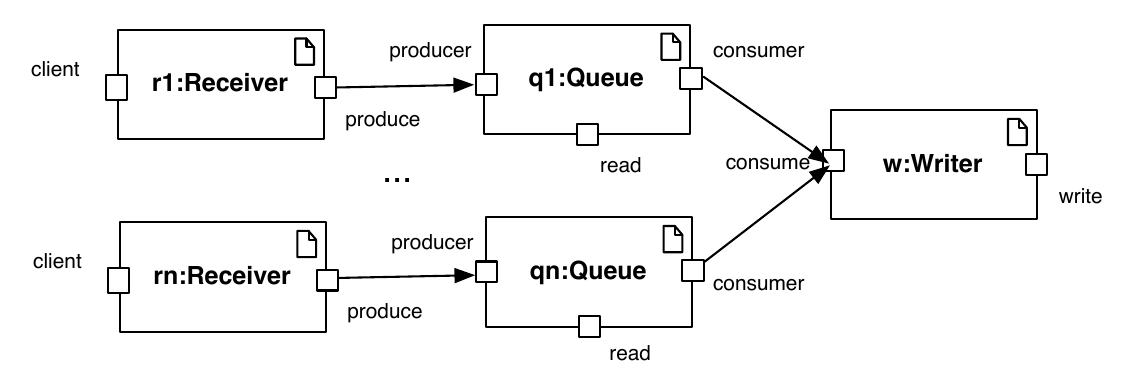
\includegraphics[width=120mm]{graphite-carbon}
    \end{center}

    \optionA{A performance scenario associated with the throughput of writing data points to disk.}
    \optionB{A performance scenario associated with the latency of writing data points to disk.}
    \optionC{An availability scenario associated with a fault in the \emph{Carbon} component.}
    \optionD{A usability scenario.}
 \putOptions
\end{ClosedQuestion}
}

\newcommand{\qGraphiteAvailabilityScenario}{
\begin{ClosedQuestion}
    In the context of the \emph{Graphite} case study, consider the following view that represents the internal behavior of the \emph{Carbon} component, where the components \texttt{r1,... , rn, w} are threads and \texttt{q1, ..., qn} are buffers. The port \emph{read}, which provides an interface to read the data points stored in the queue, can be used, in an enrichment of the view, to illustrate
    
    \begin{center}
       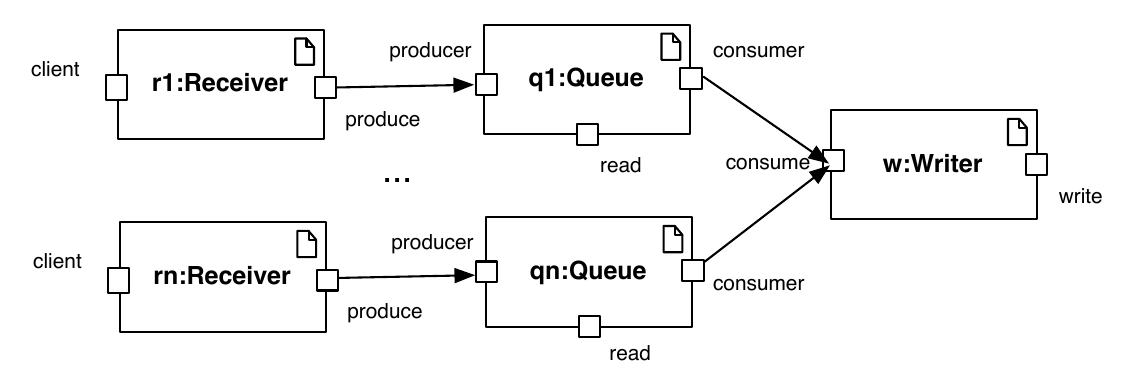
\includegraphics[width=120mm]{graphite-carbon}
    \end{center}

    \optionA{A modifiability scenario the \emph{Graphite} system.}
    \optionB{A usability scenario of the \emph{Graphite} system.}
    \optionC{A performance scenario of the \emph{Graphite} system.}
    \optionD{An availability scenario of the \emph{Graphite} system.}
 \putOptions
\end{ClosedQuestion}
}

\newcommand{\qGraphiteWebapp}{
\begin{ClosedQuestion}
    In the context of the \emph{Graphite} case study, consider the following application-specific types that are used in a view to represent the internal behavior of the \emph{Webapp} component. 
    
    \begin{center}
       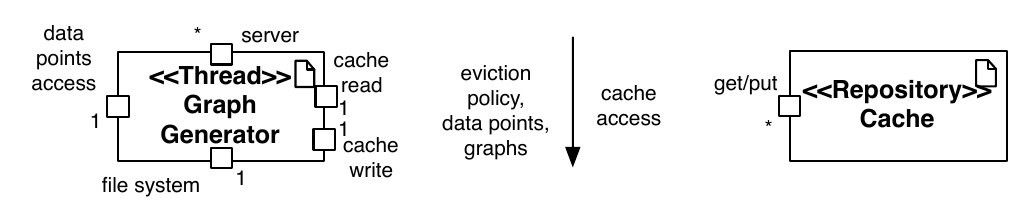
\includegraphics[width=120mm]{graphite-webapp}
    \end{center}
    
    This view can show that the architecture fulfills  

    \optionA{A modifiability scenario the \emph{Graphite} system.}
    \optionB{A usability scenario of the \emph{Graphite} system.}
    \optionC{A single performance scenario of the \emph{Graphite} system.}
    \optionD{At least two performance scenarios of the \emph{Graphite} system.}
 \putOptions
\end{ClosedQuestion}
}



% The Architecture of the Morrison's OrderPad and Silk

\newcommand{\qOrderPadPortability}{
\begin{ClosedQuestion}
    Consider the architecture of the Morrison's OrderPad. The decision whether use a Native application or HTML5 for the implementation of the client in the Pad was taken because
    
    \optionA{HTML5 provides better portability qualities.}
    \optionB{Native applications provide better modifiability qualities.}
    \optionC{HTML5 provides better usability qualities.}
    \optionD{Native applications provide better support for working offline.}
 \putOptions
\end{ClosedQuestion}
}

\newcommand{\qSilk}{
\begin{ClosedQuestion}
    In the Amazon Silk browser  
    
    \optionA{A request for a web page corresponds to a peer-to-peer interaction between all the web components containing the resources.}
    \optionB{Web pages are explicitly cached on the browser to optimize accesses.}
    \optionC{A request for a web page corresponds to requesting a service from the amazon cloud.}
    \optionD{It is possible to customize the number of threads that run in the mobile device.}
 \putOptions
\end{ClosedQuestion}
}


\newcommand{\qOrderPadIterative}{
\begin{ClosedQuestion}
    Consider the architecture of the Morrison's OrderPad. In the description of the system can be read:
    
    \begin{quote}
        The pilot version included some architectural short-cuts that would not work with the full complement of stores. One of these was using a file-transfer to send data to the mainframe rather than MQ, which wouldn't perform well once many stores were active.
    \end{quote}
    
    This approach means that
    
    \optionA{Performance was traded for easy of development to reduce the overall development costs.}
    \optionB{An iterative development was followed, which allowed more time to develop a connector with good performance in the latter stages of the project.}
    \optionC{Performance was traded for the availability quality.}
    \optionD{An incremental development was followed, which allowed to have the system in production without being necessary to export all the information to the mainframe.}
 \putOptions
\end{ClosedQuestion}
}



% Microservices

\newcommand{\qMicroservicesOne}{
\begin{ClosedQuestion}
    Consider the architectural solutions for microservices architectures that use the event sourcing technique. This technique has the following advantage 
            
    \optionA{Simplifies the evolution of the event schema.}
    \optionB{Simplifies the query operations in  the event store.}
    \optionC{Allows the querying of a past state.}
    \optionD{Provides a programming model developers are familiar with.}
 \putOptions
\end{ClosedQuestion}
}

\newcommand{\qMicroservicesTwo}{
\begin{ClosedQuestion}
    Suppose that an architect needs to decide whether to follow a modular monolith architecture or a microservices architecture for a new large system. The system to be developed has a complex logic and high volume of requests. 
            
    \optionA{She should decide to use a microservices architecture to improve the scalability of the system.}
    \optionB{She should decide to use a modular monolith architecture to reduce the cost of development, because developers will not need to define intermediate states for the transactional execution of the business logic.}
    \optionC{She should try to split the system in parts in order to isolate the complex business logic and use the two architectural approaches accordingly.}
    \optionD{She should give up because it is not possible to have the two approaches in a singe architecture.}
 \putOptions
\end{ClosedQuestion}
}

\newcommand{\qMicroservicesThree}{
\begin{ClosedQuestion}
    Consider the architectural solutions for microservices architectures that use the Command Query Responsibility Segregation (CQRS) technique in the context of Event Sourcing. This technique has the following disadvantage 
            
    \optionA{Does not allow optimizations according to the type of query.}
    \optionB{Does not support independent scalability according to the type of operation.}
    \optionC{Reads may not be consistent with the most recent write.}
    \optionD{Querying the event sourcing becomes more complex.}
 \putOptions
\end{ClosedQuestion}
}




% Third Mini-test

% Module styles

\newcommand{\qModuleStylesOne}{
  \begin{ClosedQuestion}
      Suppose that in the development of an enterprise application (which needs to access a
      database) it was decided to use the FenixFramework library to simplify the development
      of the data access code. Which architectural style is the most adequate to represent this
      decision?
      
      \optionA{The Aspects style.}
      \optionB{The Generalisation style.}
      \optionC{The Decomposition style.}
      \optionD{The Shared-data style.}
    \putOptions

% Resposta: C
  \end{ClosedQuestion}
}

\newcommand{\qUsesOne}{
\begin{ClosedQuestion}
  Which
  architectural style is 
  adequate for planning incremental
  releases?

  \optionA{The Decomposition style.}
  \optionB{The Generalisation style.}
  \optionC{The Uses style.}
  \optionD{The Aspects style.}
  \putOptions
\end{ClosedQuestion}
}

\newcommand{\qLayeredAspectsDataModelOne}{
\begin{ClosedQuestion}
  In a layered architecture composed by four layers, where the topmost
  layer is the layer number 1 and the bottommost layer is the layer
  number 4, which of the layers is more modifiable?

    \optionA{Layer 1.}
    \optionB{Layer 4.}
    \optionC{In a layered architecture all layers are equally modifiable.}
    \optionD{Modifiability is not made easier by a layered architecture.}
  \putOptions
\end{ClosedQuestion}
}


% Adventure Builder Module Viewtype

\newcommand{\qAdventureBuilderModuleOne}{
\begin{ClosedQuestion}
    Consider the following modifiability scenario for the Adventure Builder system 
    
    \begin{quote}
        A new business partner (airline, lodging, or activity provider) that uses its own web services interface is added to the system in no more than 10 person-days of effort for the implementation. The business goal is easy integration with new business partners.
    \end{quote}
    
    and the following architectural view
    
    \begin{center}
        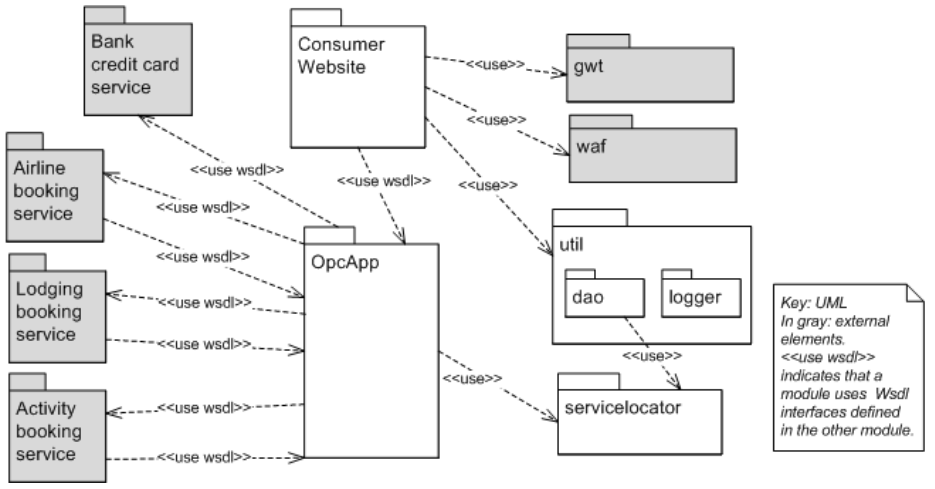
\includegraphics[width=95mm]{AdventureBuilderModule}
    \end{center}
    
    \optionA{The view does not address the scenario}
    \optionB{The view addresses the scenario because it separates the \texttt{Consumer Website} module from the \texttt{OpcApp} module.}
    \optionC{The view addresses the scenario because it separates the modules that represent the interfaces a new business partner has to implement.}
    \optionD{The view addresses the scenario because the \texttt{Consumer Website} module does not use the interfaces a new business partner has to implement.}
 \putOptions
\end{ClosedQuestion}
}

\newcommand{\qAdventureBuilderModuleTwo}{
\begin{ClosedQuestion}
    Consider the following availability scenario for the Adventure Builder system 
    
    \begin{quote}
        The Consumer Web site is available to the user 24x7. If an instance of OPC application fails, the fault is detected and the system administrator is notified in 30 seconds; the system continues taking order requests; another OPC instance is created; and data remains in consistent state.
    \end{quote}
    
    and the following architectural view
    
    \begin{center}
        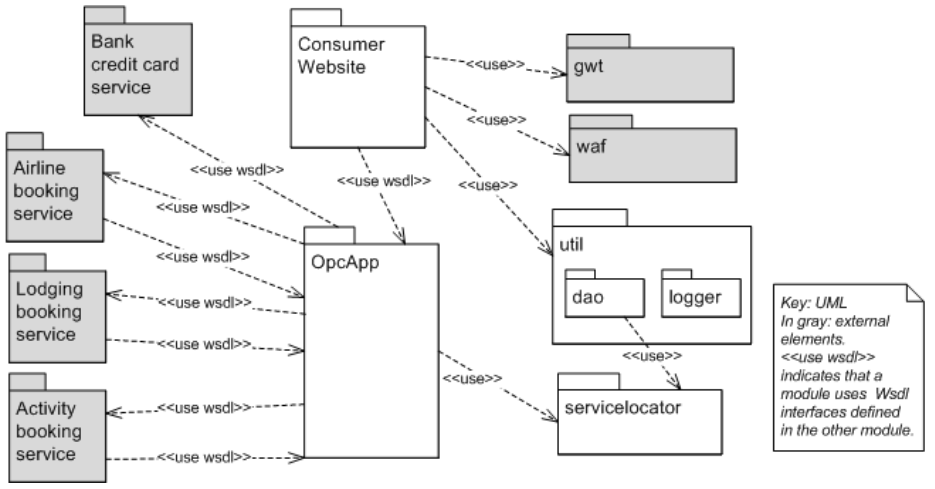
\includegraphics[width=95mm]{AdventureBuilderModule}
    \end{center}
    
    \optionA{The view does not address the scenario}
    \optionB{The view addresses the scenario because the uses relation between the \texttt{Consumer Website} module and the \texttt{OpcApp} module has the require properties.}
    \optionC{The view addresses the scenario because it separates the modules that represent the interfaces a new business partner has to implement.}
    \optionD{The view addresses the scenario because the \texttt{Consumer Website} module uses the \texttt{gwt} and \texttt{waf} modules.}
 \putOptions
\end{ClosedQuestion}
}

\newcommand{\qAdventureBuilderModuleThree}{
\begin{ClosedQuestion}
    Consider the following performance/scalability scenario for the Adventure Builder system 
    
    \begin{quote}
        Up to 500 users click to see the catalog of adventure packages following a random distribution over 1 minute; the system is under normal operating conditions; the maximal latency to serve the first page of content is under 5 seconds; average latency for same is less than 2 seconds. If required, the system should easily support an increase in the number of simultaneous requests while maintaining the same latency per request.
    \end{quote}
    
    and the following architectural view
    
    \begin{center}
        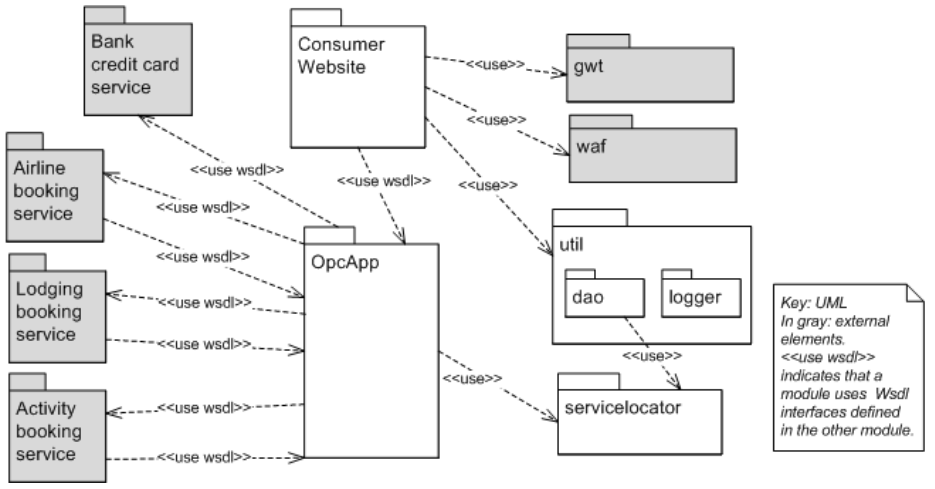
\includegraphics[width=95mm]{AdventureBuilderModule}
    \end{center}
    
    \optionA{The view does not address the scenario.}
    \optionB{The view addresses the scenario because it separates the \texttt{Consumer Website} module from the \texttt{OpcApp} module to allow the execution of the \texttt{Consumer Website} module in a component that can have multiple copies of computation.}
    \optionC{The view addresses the scenario because it separates the modules that represent the interfaces a new business partner has to implement.}
    \optionD{The view addresses the scenario because the \texttt{Consumer Website} module uses the \texttt{gwt} and \texttt{waf} modules.}
 \putOptions
\end{ClosedQuestion}
}



% Component-and-connector viewtype

\newcommand{\qInterfaceDelegation}{
\begin{ClosedQuestion}
    Consider the concept of interface delegation 
        
    \optionA{It corresponds to a particular case of a specialization in a generalization view.}
    \optionB{It represents a relation between a connector's role and a port of one of its internal components.}
    \optionC{It represents a relation between a component's port and a port of one of its internal components.}
    \optionD{It represents a relation between a component's port and a connector's role.}
 \putOptions
\end{ClosedQuestion}
}

\newcommand{\qConnectorAttach}{
\begin{ClosedQuestion}
    A connector may be attached to components of different types because
        
    \optionA{The type of a connector does not depend on the type of its roles.}
    \optionB{Components of different types may have ports of the same type.}
    \optionC{The attachment is a runtime relation which dynamically manages type compliance.}
    \optionD{The attachment between components and connectors only depends on their ports and roles types.}
 \putOptions
\end{ClosedQuestion}
}

\newcommand{\qComponentViewType}{
\begin{ClosedQuestion}
    The quality(ies) that is(are) more relevant to views of the component-and-connector viewtype is(are):
        
    \optionA{Modifiability.}
    \optionB{Availability and Performance.}
    \optionC{Testability and Modifiability.}
    \optionD{Maintainability and Availability.}
 \putOptions
\end{ClosedQuestion}
}


% Component-and-connector styles

\newcommand{\qPipeFilterComposition}{
\begin{ClosedQuestion}
    The Pipe-and-Filter style allows composition of filters 

    \optionA{But when the filters are executed sequentially the composition power is reduced.}
    \optionB{Which improves modifiability, because filters are decoupled through pipes.}
    \optionC{But the size of buffers may reduce the composition power.}
    \optionD{And filters do not have to agree on the data formats.}
 \putOptions
\end{ClosedQuestion}
}

\newcommand{\qPublishSubscribe}{
\begin{ClosedQuestion}
    In the Publish-Subscribe architectural style 
    
    \optionA{A component can subscribe to events.}
    \optionB{All the published events are received by their subscribing components.}
    \optionC{The events should be received by the same order they are sent.}
    \optionD{The set of events types are predefined at initialization time.}
 \putOptions
\end{ClosedQuestion}
}


\newcommand{\qPeerToPeerSpace}{
\begin{ClosedQuestion}
    The Peer-to-Peer architectural style provides high scalability and availability. In the context of a file sharing system  
    
    \optionA{The file transfer has to follow the same path of nodes used to identify where the file was located.}
    \optionB{The peer initiating the request for a file needs to know where the file is located.}
    \optionC{If a peer providing a file crashes the file will not be downloaded.}
    \optionD{The price for high scalability and availability is the need to have several replicas of the files to be shared.}
 \putOptions
\end{ClosedQuestion}
}


% Adventure Builder Component-and-Connector Viewtype

\newcommand{\qAdventureBuilderComponentAndConnectorOne}{
\begin{ClosedQuestion}
    Consider the following view of the Adventure Builder system
    
    \begin{center}
        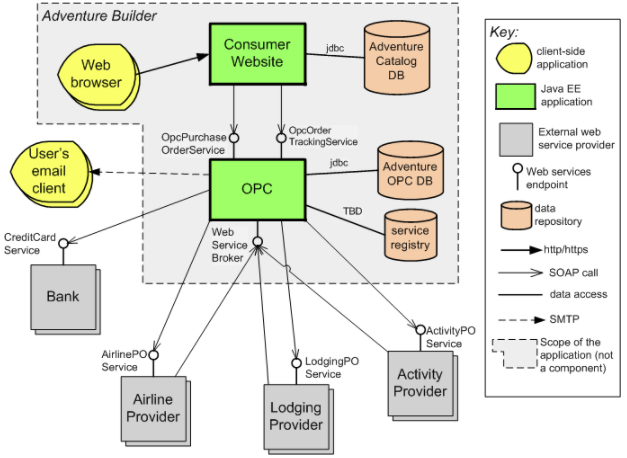
\includegraphics[width=95mm]{AdventureBuilderComponentAndConnector}
    \end{center}
    
    In this view the following architectural styles are used
    
        
    \optionA{Service-oriented architecture, and Client-server.}
    \optionB{Service-oriented architecture, and Shared-data.}
    \optionC{Service-oriented architecture, Shared-data, and Client-server.}
    \optionD{Service-oriented architecture, Shared-data, Client-server and Peer-to-peer.}
 \putOptions 
\end{ClosedQuestion}
}


\newcommand{\qAdventureBuilderComponentAndConnectorSecond}{
\begin{ClosedQuestion}
    Consider the following view of the Adventure Builder system
    
    \begin{center}
        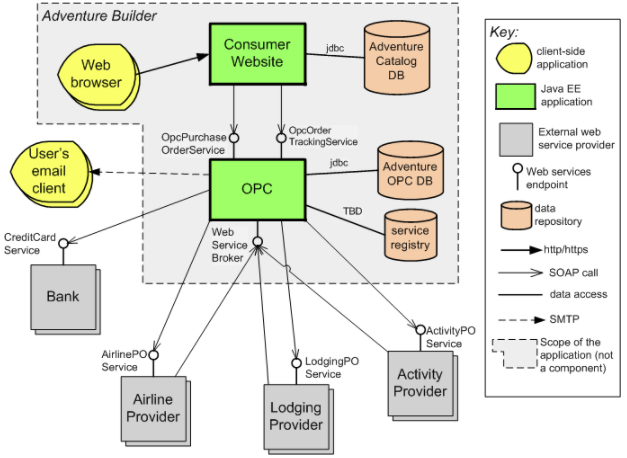
\includegraphics[width=95mm]{AdventureBuilderComponentAndConnector}
    \end{center}
    
    In this view it is possible to reason that
    
    \optionA{If the OPC crashes the Consumer Website can continue to provide service in degraded mode.}
    \optionB{If the OPC crashes the Consumer Website can continue to provide service in normal mode.}
    \optionC{If the Adventure Catalog BD crashes the Consumer Website can continue to present the Adventure Builder offers.}
    \optionD{If a Bank component is not available the OPC cannot continue to provide service.}
 \putOptions 
\end{ClosedQuestion}
}



\newcommand{\qAdventureBuilderComponentAndConnectorThird}{
\begin{ClosedQuestion}
    Consider the following view of the Adventure Builder system
    
    \begin{center}
        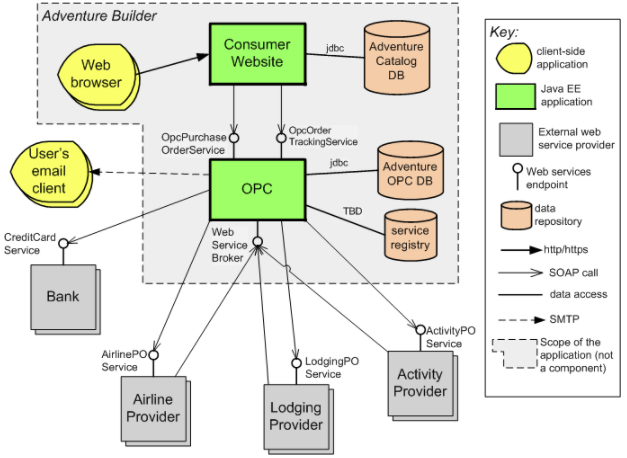
\includegraphics[width=95mm]{AdventureBuilderComponentAndConnector}
    \end{center}
    
    This view \textbf{does not} apply the architectural style
    
        
    \optionA{Client-server.}
    \optionB{Publish-subscribe.}
    \optionC{Shared-data.}
    \optionD{Peer-to-peer.}
 \putOptions 
\end{ClosedQuestion}
}



% Second Mini-test


% Availability

\newcommand{\qAvailabilityVotingFirst}{
  \begin{ClosedQuestion}
    There are several tactics to satisfy availability requirements,
    which may be applied depending on the concrete requirement that we
    want to satisfy.  Assuming that you want to detect faults of type
    \emph{response} in your system, which tactic is more adequate?

    \optionA{Ping/Echo.}
    \optionB{Retry.}
    \optionC{Voting.}
    \optionD{Passive Redundancy.}

    \putOptions

% Resposta: C
 \end{ClosedQuestion}
}

\newcommand{\qAvailabilityVotingSecond}{
  \begin{ClosedQuestion}
      The availability quality can be supported by a voting tactic in order to identify faults of

      \optionA{Programming, if the components execute modules developed by different teams.}
      \optionB{Hardware, if there is hardware redundancy.}
      \optionC{Operating Systems, if redundant components execute on top of different operating systems..}
      \optionD{All the previous options.} 
      

     \putOptions
% Resposta: D
   \end{ClosedQuestion}
}

\newcommand{\qVoting}{
\begin{ClosedQuestion}
    A voting tactic can be used to

    \optionA{Prevent a fault in hardware.}
    \optionB{Prevent a fault in software.}
    \optionC{Prevent a fault in a process.}
    \optionD{Detect a fault.}
 \putOptions
\end{ClosedQuestion}
}



% Modifiability

%4
\newcommand{\qModifiabilityOne}{
\begin{ClosedQuestion}
    The modifiability tactic Use an Intermediary between two modules
        
    \optionA{Has as main goal the reduction of the modules' size.}
    \optionB{Results in the creation of a third module that makes the original modules independent.}
    \optionC{Increases the cohesion between the two modules.}
    \optionD{May conflict with the Reduce Overhead performance tactic.}
 \putOptions 
\end{ClosedQuestion}
}

%5
\newcommand{\qModifiabilityTwo}{
\begin{ClosedQuestion}
    Consider the following scenario: \emph{A system administrator adds more copies of computation of the system, each one using a different database, and is able to do it in less than 10 minutes.}
        
    \optionA{This is a performance scenario and the measure of the response is 10 minutes latency.}
    \optionB{This is a modifiability scenario which has a defer binding tactic.}
    \optionC{This is not a modifiability scenario because the source of the stimulus cannot be a system administrator.}
    \optionD{This is a modifiability scenario and its environment design time.}
 \putOptions 
\end{ClosedQuestion}
}

%6
\newcommand{\qModifiabilityThree}{
\begin{ClosedQuestion}
    Consider the modifiability quality and the cost of change.
        
    \optionA{A low cost of change may imply a high cost of development.}
    \optionB{A low cost of change implies a low cost of development, because changing the code is part of development.}
    \optionC{There is no relation between the cost of change and the cost of development.}
    \optionD{The cost of change is higher if it occurs at runtime.}
 \putOptions 
\end{ClosedQuestion}
}




% Designing-an-Architecture

\newcommand{\qFenixADD}{
\begin{ClosedQuestion}
    When applying Attribute-Driven Design (ADD) to the FenixEdu system the creation of a view where there are redundant web servers, load balancers and database servers 

    \optionA{Results from a utility tree for performance.}
    \optionB{Results from a single availability scenario.}
    \optionC{Results from the application of a single ADD iteration.}
    \optionD{Results from the application of several ADD iterations.}
 \putOptions
\end{ClosedQuestion}
}


\newcommand{\qLowArchitecturalImpact}{
\begin{ClosedQuestion}
    Consider an architecturally significant requirement (ASR) that has a low impact on the architecture but a high business value

    \optionA{This ASR can easily be supported by the architecture because it has little effect in the architecture.}
    \optionB{This ASR requires a specific architectural design because it profoundly affects the architecture.}
    \optionC{The cost of meeting the ASR after development starts is too high.}
    \optionD{Any ASR that has a high business value cannot have a low architecture impact because it needs to be supported by the architecture.}
 \putOptions
\end{ClosedQuestion}
}

\newcommand{\qIterativeDesign}{
\begin{ClosedQuestion}
    Designing an architecture

    \optionA{Is driven by functional requirements.}
    \optionB{Is done in a single step, after all the tactics were identified.}
    \optionC{Is a top-down process where a initial decomposition is chosen and it is successively decomposed without changing the initial decisions.}
    \optionD{Is an iterative process where architectural designs are proposed as hypothesis and tested.}
 \putOptions
\end{ClosedQuestion}
}




% Module Viewtype

\newcommand{\qModuleViewtypeOne}{
\begin{ClosedQuestion}
    Consider the Decomposition architectural style of the Module viewtype
        
    \optionA{Its main goal is to establish the reusability qualities of the architecture.}
    \optionB{Project managers are not interested in views that use this style because it lacks the necessary level of detail.}
    \optionC{Views of this type are mostly useful to guide the testing of the system.}
    \optionD{There should be at least one view of the system using this architectural style.}
 \putOptions 
\end{ClosedQuestion}
}

\newcommand{\qDecomposition}{
\begin{ClosedQuestion}
    The Decomposition architectural style of the Module viewtype 
    
    \optionA{Is applied only once at the beginning of the architectural design process.}
    \optionB{Is applied at the begin of the architectural design process but may be necessary to redo it later.}
    \optionC{Is mostly driven by the security attribute quality.}
    \optionD{Follows a bottom-up decomposition process of the system.}
 \putOptions
\end{ClosedQuestion}
}

\newcommand{\qArchitecturalViews}{
\begin{ClosedQuestion}
  A software system is usually described using different architectural views

  \optionA{Each view contains a single architectural style.}
  \optionB{Views need to contain more than one architectural style.}
  \optionC{A view may not contain any architectural style.}
  \optionD{None of the above.}
  \putOptions
  \end{ClosedQuestion}
}



% Graphite 

\newcommand{\qGraphiteComposerUIPerformance}{
  \begin{ClosedQuestion}
      The \emph{Composer UI} component of Graphite system, described as - \emph{Graphite's Composer UI provides a point-and-click method to create a graph from which you can simply copy and paste the URL} - to be effective needs to show to the user the changes she performs in the graph such that she has immediate feedback whenever she clicks on a option. To do so, the architecture needs to include

    \optionA{Task Model tactics.}
    \optionB{System Model tactics.}
    \optionC{performance tactics.}
    \optionD{User Model tactics.} 

     \putOptions
% Resposta: C
   \end{ClosedQuestion}
}


\newcommand{\qGraphiteScenarioTacticsOne}{
  \begin{ClosedQuestion}
    In the Graphite system the component \emph{carbon} provides to \emph{webapp} components an access interface to the \emph{buffers} in order to improve the quality of

    \optionA{Performance.}
    \optionB{Interoperability.}
    \optionC{Availability.}
    \optionD{Security.}

     \putOptions
% Resposta: C
   \end{ClosedQuestion}
}

\newcommand{\qGraphiteReliability}{
\begin{ClosedQuestion}
    In the Graphite system description can be read:
    
    \begin{quote}
        We've got 600,000 metrics that update every minute and we're assuming our storage can only keep up with 60,000 write operations per minute. This means we will have approximately 10 minutes worth of data sitting in carbon's queues at any given time. To a user this means that the graphs they request from the Graphite webapp will be missing the most recent 10 minutes of data.
    \end{quote}

    \optionA{The quality addressed is availability and transactions tactic is required to solve the problem.}
    \optionB{The quality addressed is performance and a limit event response is required to solve the problem.}
    \optionC{The quality addressed is availability and a voting design tactic is required to solve the problem.}
    \optionD{The quality addressed is performance and a maintain multiple copies of data design tactic is required to solve the problem.}
 \putOptions
\end{ClosedQuestion}
}




% First Mini-test

% The architecture elevator

\newcommand{\qElevatorCommon}{
\begin{ClosedQuestion}
    In the Architect Elevator article by Gregor Hohpe can be read:
    
    \begin{quote}
        Finding the appropriate context requires the architect to visit many floors of the organization.
    \end{quote}
    
    This sentence reflects the fact that an architecture is

    \optionA{The result of decisions that are made at the "upper floors" of the organization}
    \optionB{The sole decision of an architect}
    \optionC{A common understanding to be achieve among all the system stakeholders}
    \optionD{A set of software elements and their relations}
 \putOptions
\end{ClosedQuestion}
}

\newcommand{\qElevatorInteroperability}{
\begin{ClosedQuestion}
    In the Architect Elevator article by Gregor Hohpe can be read:
    
    \begin{quote}
        Once a developer approached our architecture team with an application that had "significant scalability demands". A quick look at the architecture diagram revealed numerous components communicating via XML messages. When I pointed out that this may be the very reason for the performance concerns, I was quickly informed that this was an architecture decision and couldn't be changed. Assuming the architects are smart and well-intentioned, they may have thought about interoperability when they made this decision but may be unaware of the negative impact on run-time performance and development velocity.
    \end{quote}
    
    From this sentence we can conclude that
        
    \optionA{Interoperability is a quality that as lower priority than performance}
    \optionB{Scalability should be the quality to be achieved first by any architecture}
    \optionC{That the use of XML technology for interoperability is not a correct decision}
    \optionD{None of the above}
 \putOptions
\end{ClosedQuestion}
}

\newcommand{\qElevatorDevops}{
\begin{ClosedQuestion}
    In the Architect Elevator article by Gregor Hohpe can be read:
    
    \begin{quote}
        A lot of large companies have discovered the benefits of cloud computing but see it mainly as an infrastructure topic. I feel that's misguided: being able to get compute resources more quickly and cheaply is useful, but the real business benefit lies in a fully automated tool chain that minimizes the time in which a normal code change can go into production. Not quite coincidentally, this is my favorite definition of DevOps.
    \end{quote}
    
    In the author's opinion
        
    \optionA{Time to market is the most important impact of cloud computing in an architecture}
    \optionB{Reduction of cost is the most important impact of cloud computing in an architecture}
    \optionC{Cloud computing has impact on the business but it is not an architectural aspect}
    \optionD{Using cloud computing we cannot delay some architectural decisions}
 \putOptions
\end{ClosedQuestion}
}


% Microservices

\newcommand{\qMicroservicesProject}{
\begin{ClosedQuestion}
    In the description of the Microservices Architecture by James Lewis and Martin Fowler can be read:
    
    \begin{quote}
        The microservice approach to division ..., splitting up into services organized around business capability. Such services take a broad-stack implementation of software for that business area, including user-interface, persistent storage, and any external collaborations. Consequently the teams are cross-functional, including the full range of skills required for the development: user-experience, database, and project management.
    \end{quote}
    
    Considering the architecture influence cycle, which influence factor it is being considered?

    \optionA{Commercial}
    \optionB{Technical}
    \optionC{Project}
    \optionD{Professional}
 \putOptions 
\end{ClosedQuestion}
}

\newcommand{\qMicroservicesModularity}{
\begin{ClosedQuestion}
    In the description of the Microservices Architecture by James Lewis and Martin Fowler can be read:
    
    \begin{quote}
        As well as the fact that services are independently deployable and scalable, each service also provides a firm module boundary, even allowing for different services to be written in different programming languages. They can also be managed by different teams.
    \end{quote}
    
    Which is not necessarily an advantage of being independently deployable and scalable?

    \optionA{Performance}
    \optionB{Availability}
    \optionC{Modifiability}
    \optionD{Time to market}
 \putOptions 
\end{ClosedQuestion}
}

\newcommand{\qMicroservicesConsistency}{
\begin{ClosedQuestion}
    In the description of the Microservices Architecture by James Lewis and Martin Fowler can be read:
    
    \begin{quote}
        Decentralizing responsibility for data across microservices has implications for managing updates. The common approach to dealing with updates has been to use transactions to guarantee consistency when updating multiple resources. This approach is often used within monoliths.
    \end{quote}
    
    What is the impact of decentralizing responsibility for data across microservices?

    \optionA{The need to use a two-phase commit protocol}
    \optionB{The need to have a tight integration of the development teams}
    \optionC{The need to have eventual consistency and compensating operations}
    \optionD{The need to deploy all the microservices simultaneously}
 \putOptions 
\end{ClosedQuestion}
}


% Architectures for scalable web applications

\newcommand{\qScalablePartitioning}{
\begin{ClosedQuestion}
    Consider the following figure that presents an architectural view of an \emph{Image Hosting Application} which resulted from the enrichment of another architectural view by adding another \emph{Image File Storage} pair, in the figure they are distinguished by 1 and 2. 
    
    \begin{center}
        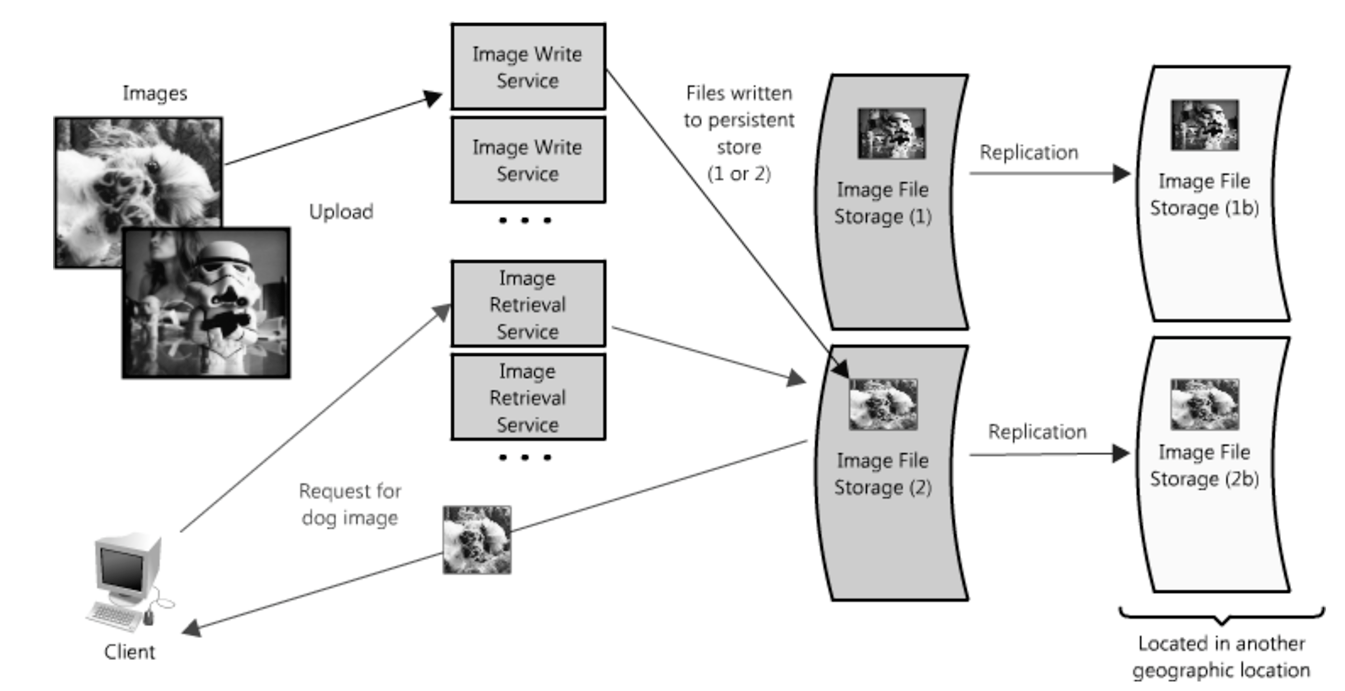
\includegraphics[width=100mm]{ScalablePartitioning}
    \end{center}
    
    Which quality results from this enrichment, that was not provided by the previous version of the architecture?
    
    \optionA{Availability of the Image Write Service, whenever one of the Image Write Service components crashes}
    \optionB{Scalability of the Image File Storage in terms of the storage capacity}
    \optionC{Availability of the Image File Storage, whenever the Image File Storage component crashes}
    \optionD{Performance of the Image Write Service}
 \putOptions 
\end{ClosedQuestion}
}

\newcommand{\qReadsAndWrites}{
\begin{ClosedQuestion}
    Consider the following figure that presents an architectural view of an \emph{Image Hosting Application}. 
    
    \begin{center}
        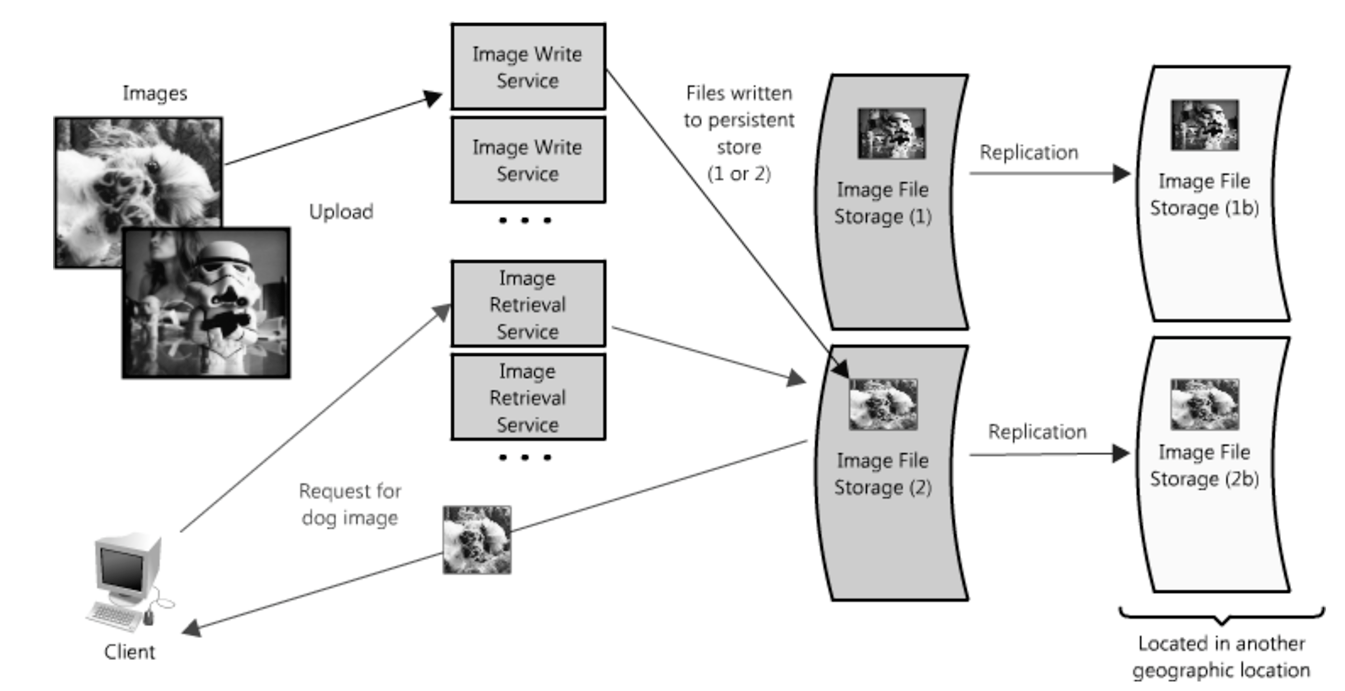
\includegraphics[width=100mm]{ScalablePartitioning}
    \end{center}
        
    \optionA{The number of Image Write Service components should be the same of the number Image Retrieval Service components}
    \optionB{The hardware where of Image Write Service components execute should have the same capabilities of the hardware where Image Retrieval Service components run}
    \optionC{Both components, the Image Write Service and the Image Retrieval Service, should be designed using an synchronous model of interactions, where a thread is associated with each request}
    \optionD{The separation of write and retrieval services allows them do scale independently}
 \putOptions 
\end{ClosedQuestion}
}

\newcommand{\qDataStorageAvailability}{
\begin{ClosedQuestion}
    Consider the following figure that presents an architectural view of an \emph{Image Hosting Application}. 
    
    \begin{center}
        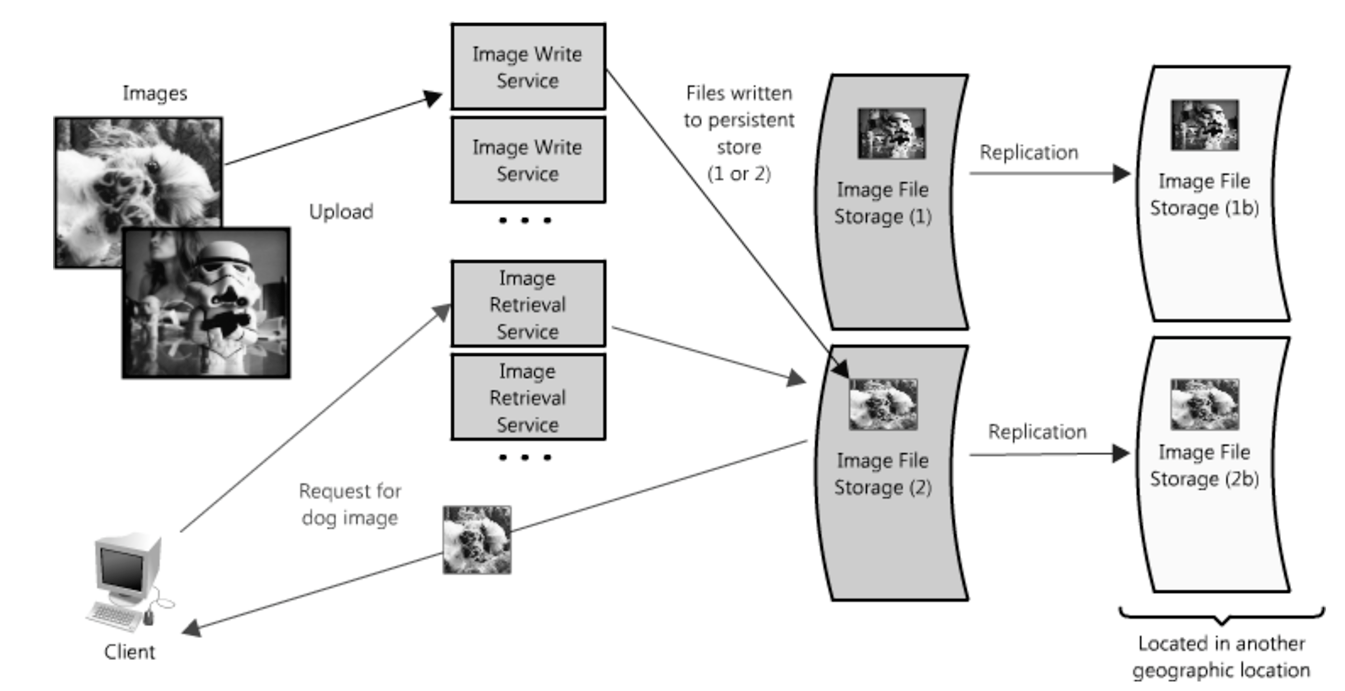
\includegraphics[width=100mm]{ScalablePartitioning}
    \end{center}
    
    The replication between the Image File Storage \emph{n} and Image File Storage \emph{nb}
        
    \optionA{Provides the quality of availability}
    \optionB{Provides the quality of performance}
    \optionC{Provides the quality of modifiability}
    \optionD{Does not provide any additional quality}
 \putOptions 
\end{ClosedQuestion}
}



\newcommand{\qQueuesQualities}{
\begin{ClosedQuestion}
    Consider the following figure that presents a Queue where client applications write their requests to be processed by a server.
    
    \begin{center}
        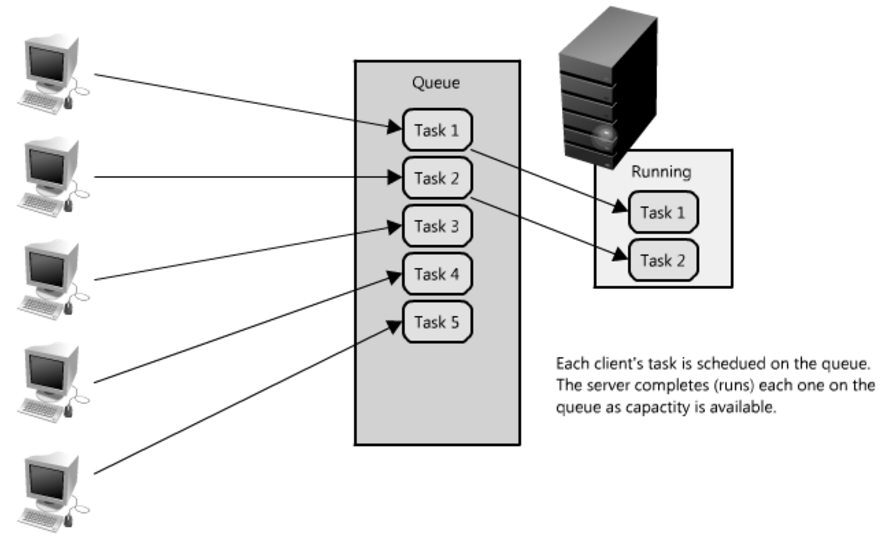
\includegraphics[width=100mm]{Queues}
    \end{center}
    
    This solution \textbf{does not} provide the following quality:
    
    \optionA{Availability whenever the server running the tasks crashes, the tasks are restarted and eventually finished}
    \optionB{Performance of the tasks execution, scheduling of tasks can be optimized for the particular context of the system}
    \optionC{Performance of the services being executed by the clients, they can execute other actions while waiting for the response}
    \optionD{Simple programming model, the clients only need to concern about the business logic of the application, the remote services are transparent}
 \putOptions 
\end{ClosedQuestion}
}

\newcommand{\qQueuesSyncAndAsync}{
\begin{ClosedQuestion}
    Consider the following figure that presents a Queue where client applications write their requests to be processed by a server (asynchronous) and compare with another architectural design (synchronous) where a thread is associated with each request.
    
    \begin{center}
        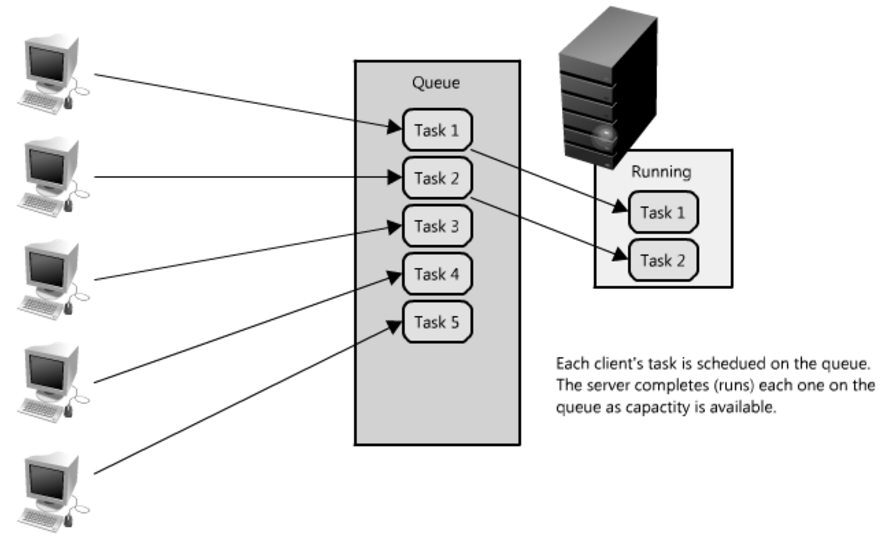
\includegraphics[width=100mm]{Queues}
    \end{center}
        
    \optionA{The synchronous solution requires less memory than asynchronous solution}
    \optionB{The asynchronous solution can support a larger number of simultaneous requests}
    \optionC{In the synchronous solution a task can be associated, during its execution, with different execution entities, e.g. thread}
    \optionD{In the asynchronous solution a task is always associated, during its execution, with the same execution entity, e.g. thread}
 \putOptions 
\end{ClosedQuestion}
}

\newcommand{\qQueuesCrash}{
\begin{ClosedQuestion}
    Consider the following figure that presents a Queue where client applications write their requests to be processed by a server (asynchronous) and compare with another architectural design (synchronous) where a thread is associated with each request.
    
    \begin{center}
        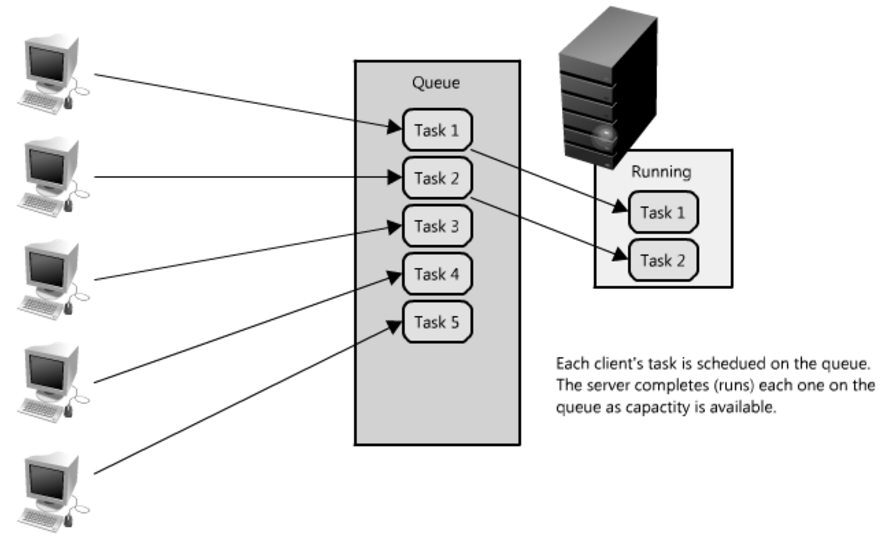
\includegraphics[width=100mm]{Queues}
    \end{center}
    
    Consider a situation where the server that processes the tasks crashes
        
    \optionA{In the synchronous solution only some of the tasks that are being executed are lost and they have to be resubmitted by the client}
    \optionB{In the asynchronous solution the tasks that are being executed are lost and they have to be resubmitted by the client}
    \optionC{In the asynchronous solution it is possible to provide an implement where the tasks being executed are finished without requiring the client to resubmitted them}
    \optionD{In the synchronous solution the tasks being executed are finished without requiring the client to resubmitted them}
 \putOptions 
\end{ClosedQuestion}
}




% Performance

\newcommand{\qPerformanceSenario}{
\begin{ClosedQuestion}
    Consider the following scenario for performance
    
    \begin{quote}
        During the enrollment period the FenixEDU system should be able to completely enroll 5.000 students in less than 30 minutes.
    \end{quote}
    
    \optionA{The source of stimulus is the FenixEDU system}
    \optionB{The stimulus is periodic}
    \optionC{The environment is overloaded}
    \optionD{The measure of the response is throughput}
 \putOptions 
\end{ClosedQuestion}
}

\newcommand{\qPerformanceTacticsOne}{
\begin{ClosedQuestion}
    Which of the following tactics is not related with the management of resources
    
    \optionA{Introduce concurrency}
    \optionB{Limit event response}
    \optionC{Maintain multiple copies of data}
    \optionD{Schedule resources}
 \putOptions 
\end{ClosedQuestion}
}

\newcommand{\qPerformanceTacticsTwo}{
\begin{ClosedQuestion}
    Which of the following tactics is not related with the control of resource demand
    
    \optionA{Manage sampling rate}
    \optionB{Bound execution times}
    \optionC{Maintain multiple copies of computation}
    \optionD{Increase resource efficiency}
 \putOptions 
\end{ClosedQuestion}
}
